\section{Exploratory landmark analysis of PDAC data}\label{appendix:landmark}

\begin{figure}[b!]
    \centering
    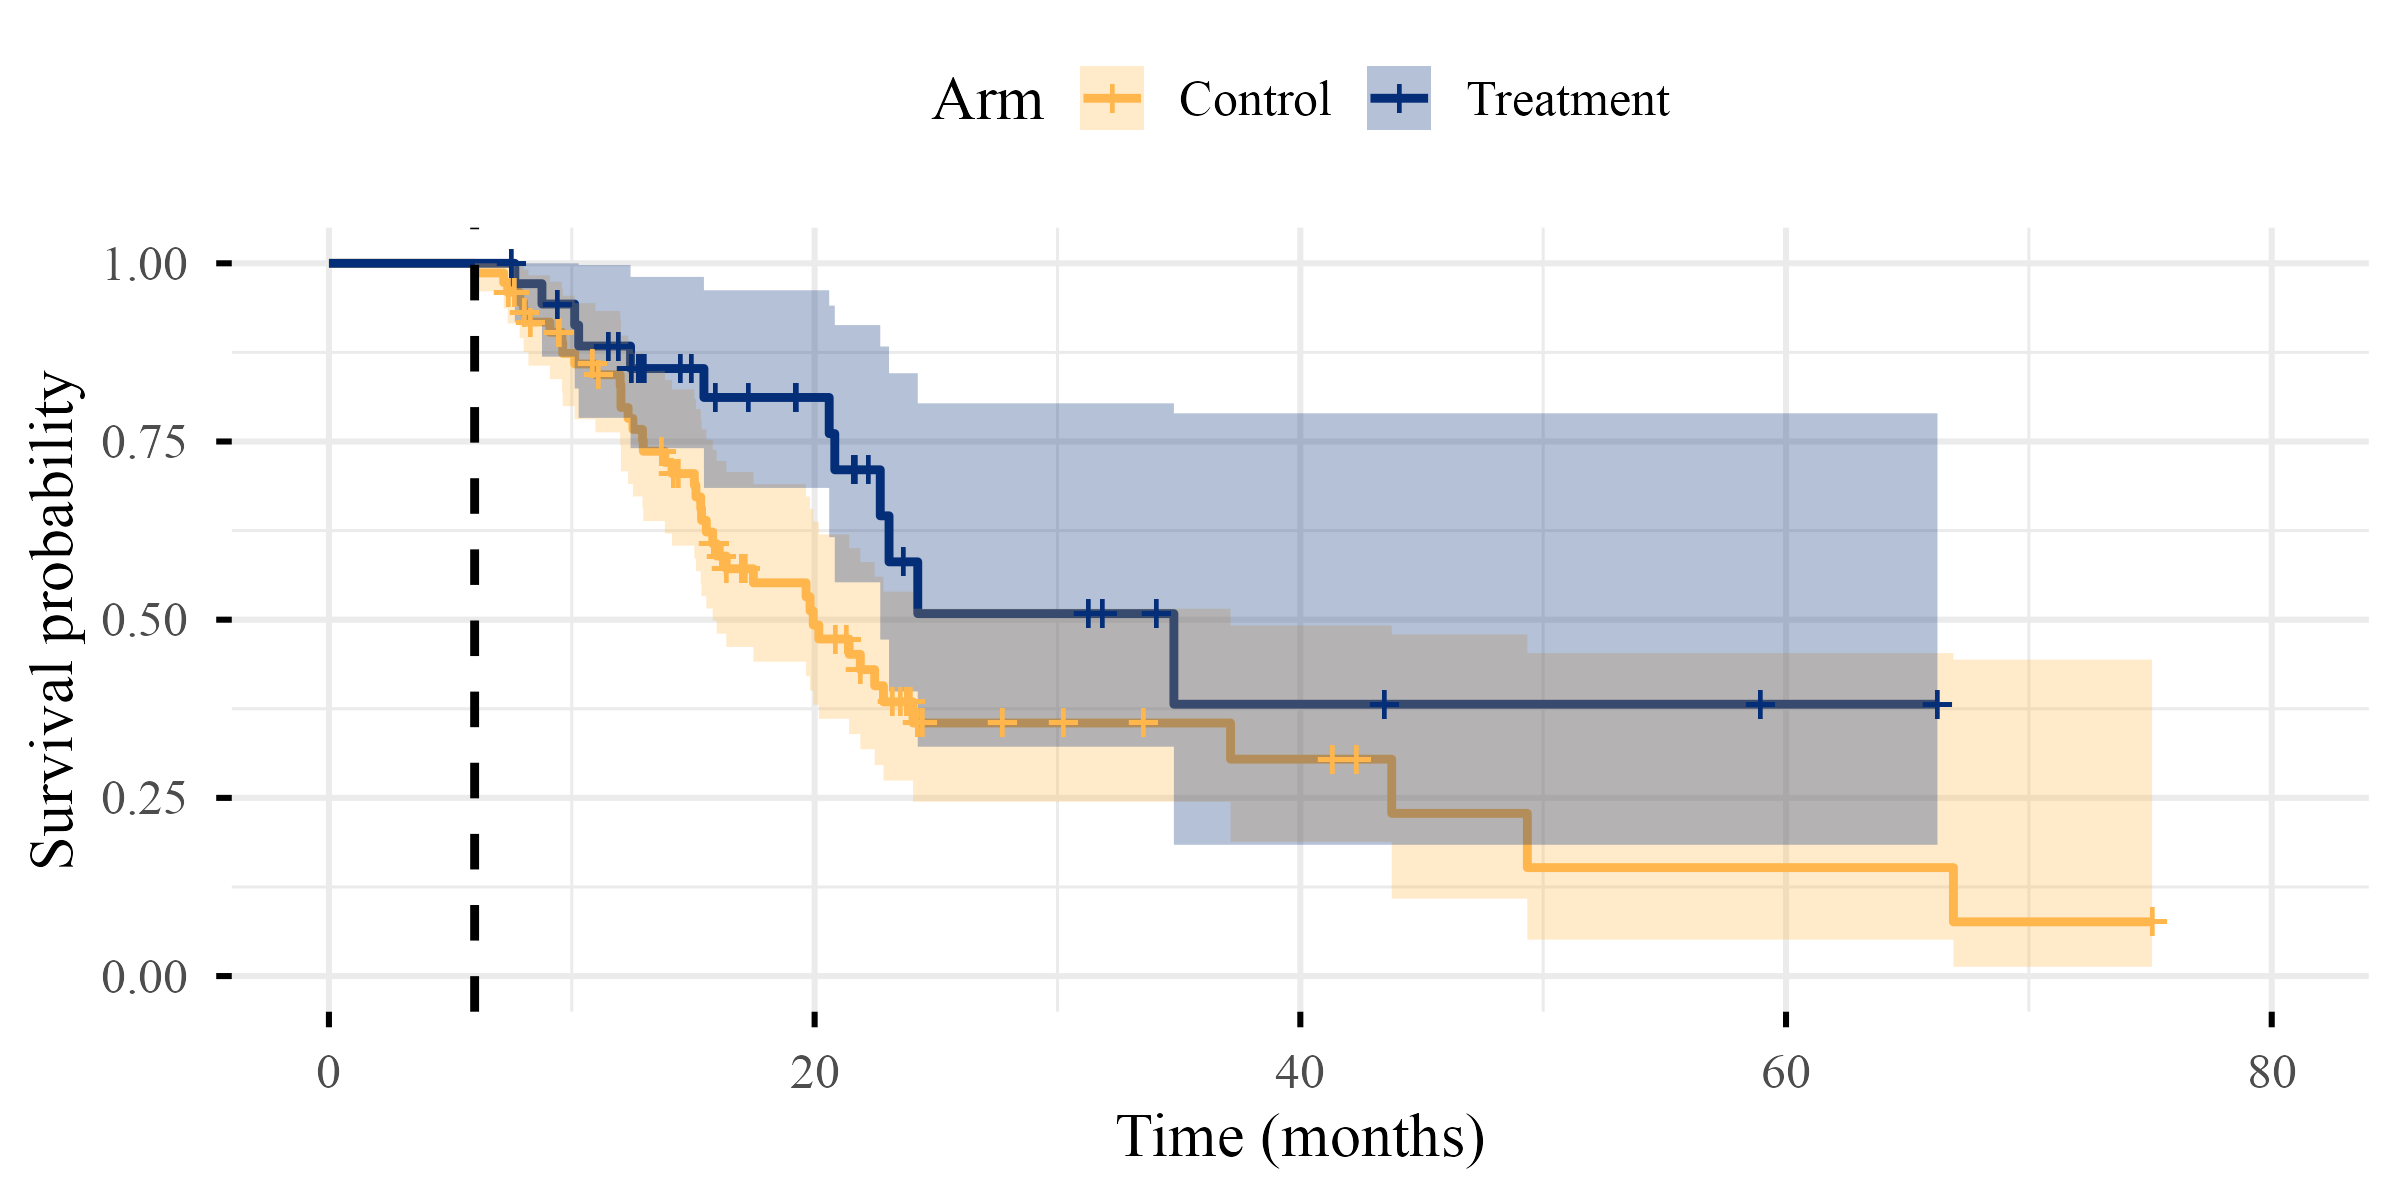
\includegraphics[width=0.7\linewidth]{KM_Landmark.png}
    \caption{Kaplan--Meier survival curves for patients with PDAC after applying the 6-month landmark analysis. The vertical dashed line indicates the landmark time.}
    \label{fig:PDAC_KaplanMeier_Landmark}
\end{figure}


We conducted a preliminary landmark analysis on the PDAC data to explore the potential impact of immortal time bias.  
Two important caveats must be emphasised. 
First, we do not have detailed information on the exact timing of adjuvant radiation therapy initiation. 
We must therefore assume that at the chosen landmark time, patients classified as controls would not have subsequently received the treatment. 
Second, we applied our original model and estimands directly to the landmark cohort without formal adaptation to a rigorous landmark analysis framework. 
The results of this analysis should be interpreted with caution and viewed primarily as an exploratory sensitivity analysis, motivating further research rather than providing definitive causal conclusions.

The landmarking approach aims to mitigate immortal time bias by conditioning on survival up to a fixed time point.
It ensures that all included patients are comparably at risk beyond the landmark time. 
This strategy has been advocated in the survival analysis literature as a pragmatic way to reduce immortal time bias \citep{vanHouwelingen2007Dynamic}. 
However, fully addressing this bias requires explicit modelling of time-dependent treatment assignment and joint survival-treatment processes. 
This was not possible with the available data.




We set the landmark time at 6 months. 
Patients not at risk at this time point were excluded.
This results in a sample of $n = 110$ patients, with 36 in the treatment group and 74 in the control group (based on the original sample used in the main analysis). 
The corresponding Kaplan--Meier survival curves are shown in Figure~\ref{fig:PDAC_KaplanMeier_Landmark}. 
We then re-estimated the causal effects using the Causal Horseshoe Forest approach described earlier.


The model achieved a concordance index of $0.75$. 
The posterior mean ATE was estimated at approximately $0.55$, with a 95\% credible interval of ($0.10$, $0.98$), as shown in Figure~\ref{fig:posterior_ATE_Landmark}. 
Posterior distributions of the individual conditional average treatment effects are displayed in Figure~\ref{fig:cate_plot_Landmark}. 
The estimated CATEs suggest a relatively homogeneous treatment effect across patients, although the wide credible intervals highlight the uncertainty due to the smaller sample size and reduced number of events after landmarking.



The landmark analysis suggests a positive average treatment effect after accounting for potential immortal time bias. 
The estimated effect is smaller than in the main analysis.
This suggests that immortal time bias may have inflated the treatment effect observed previously.
The interpretation of this analysis crucially depends on the assumption that all patients would have had the opportunity to receive and complete adjuvant radiation therapy within one year after surgery.  
Future work incorporating explicit time-dependent treatment modelling is warranted to rigorously evaluate this potential bias.

\begin{figure}[tb]
    \centering
    \begin{minipage}[ht]{0.48\linewidth}
        \centering
        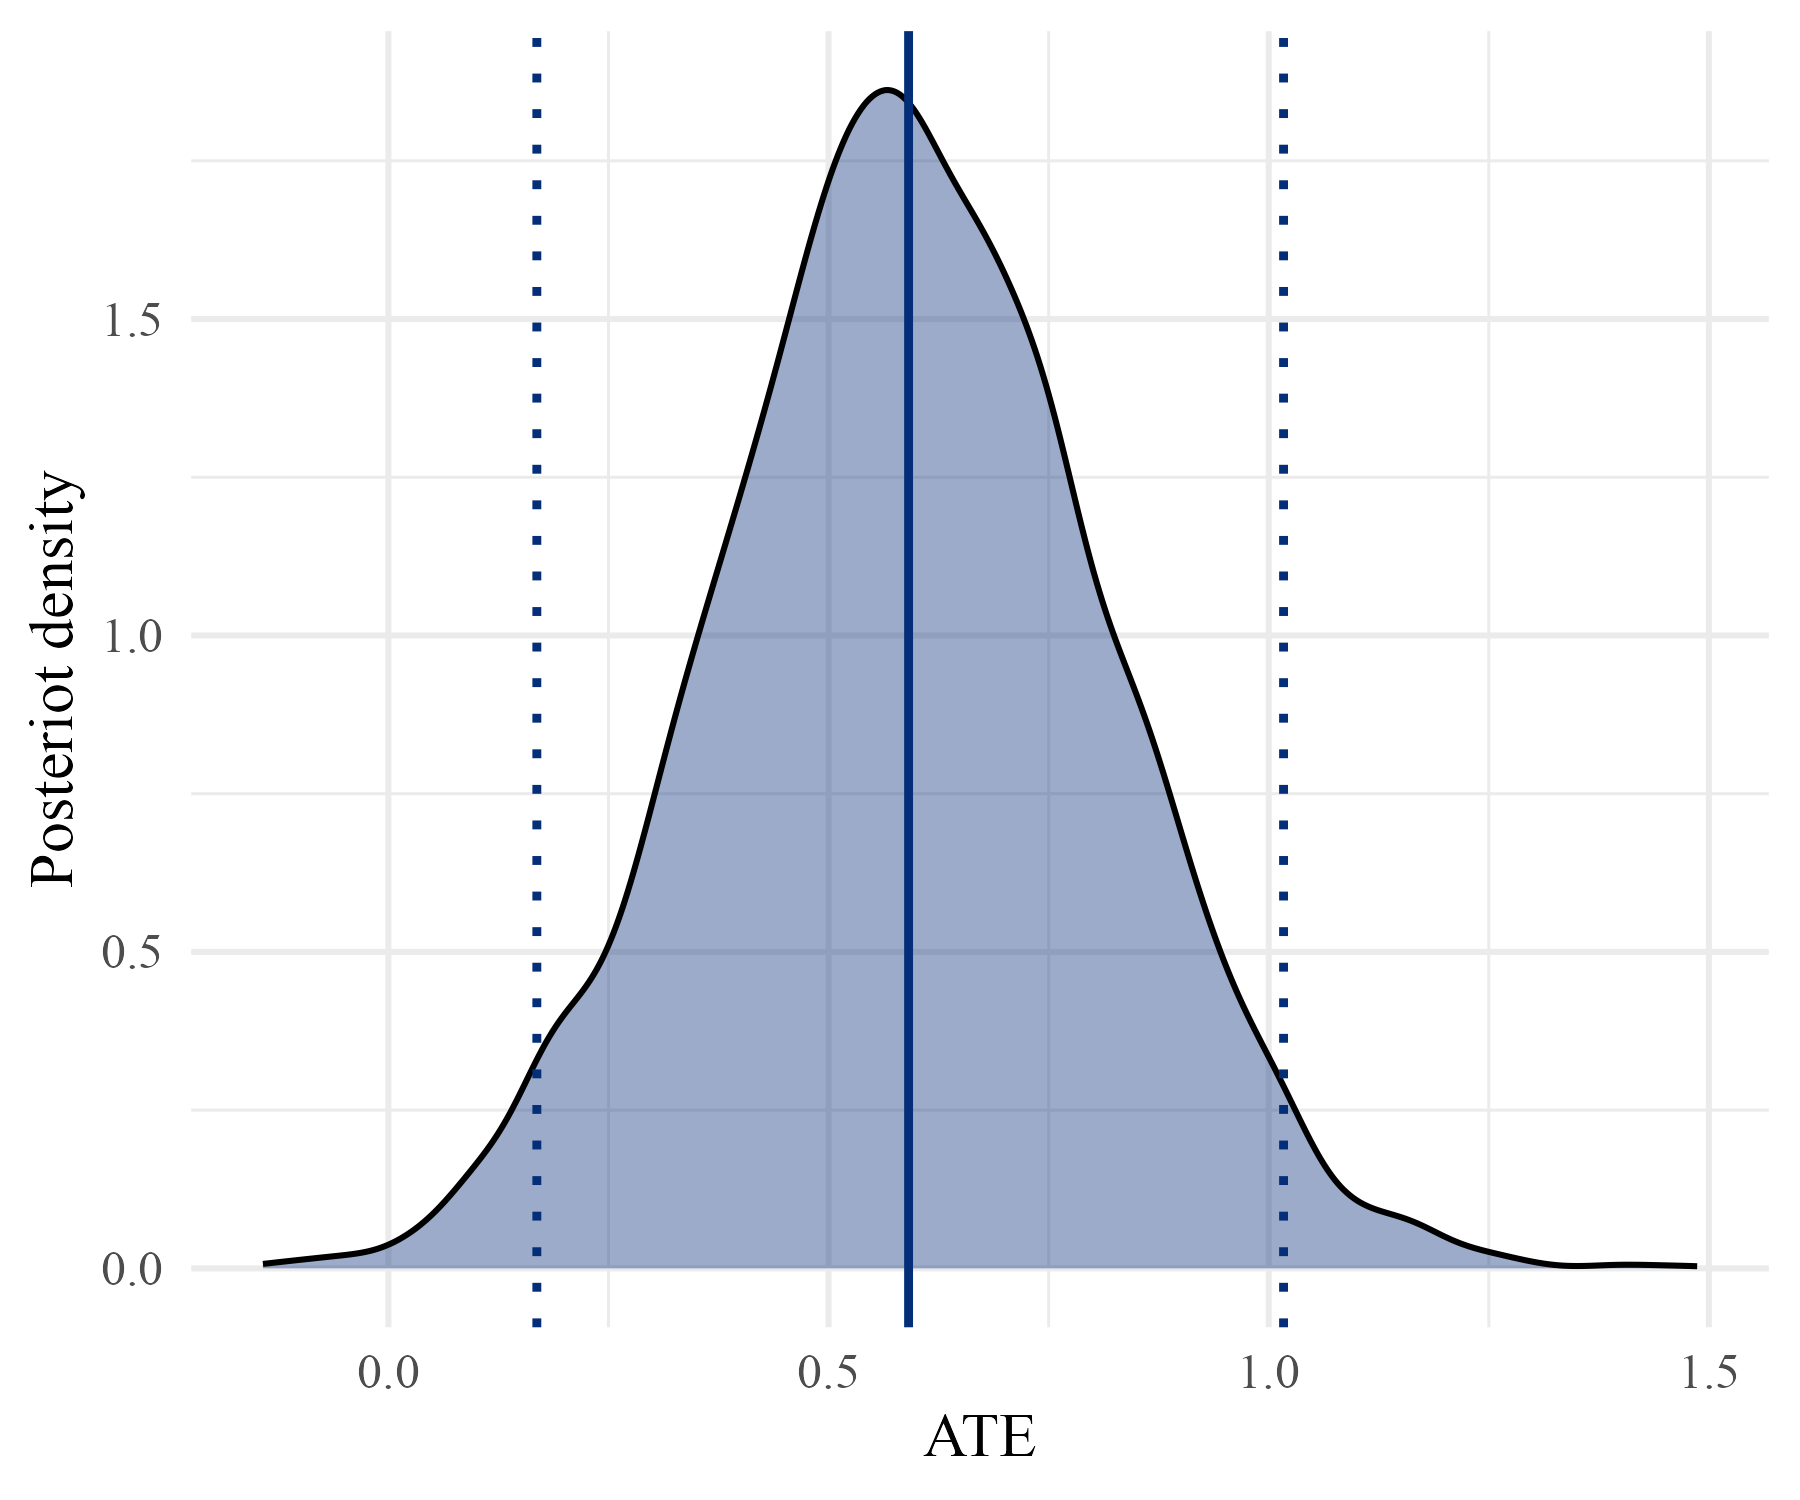
\includegraphics[width=\linewidth]{Plot_posteriorATE_Landmark.png}
        \caption{Posterior distribution of the ATE of adjuvant radiotherapy on overall survival in patients with PDAC after 6-month landmarking. The solid vertical line indicates the posterior mean, and dotted lines show the 95\% credible interval.}
        \label{fig:posterior_ATE_Landmark}
    \end{minipage}
    \hfill
    \begin{minipage}[ht]{0.48\linewidth}
        \centering
        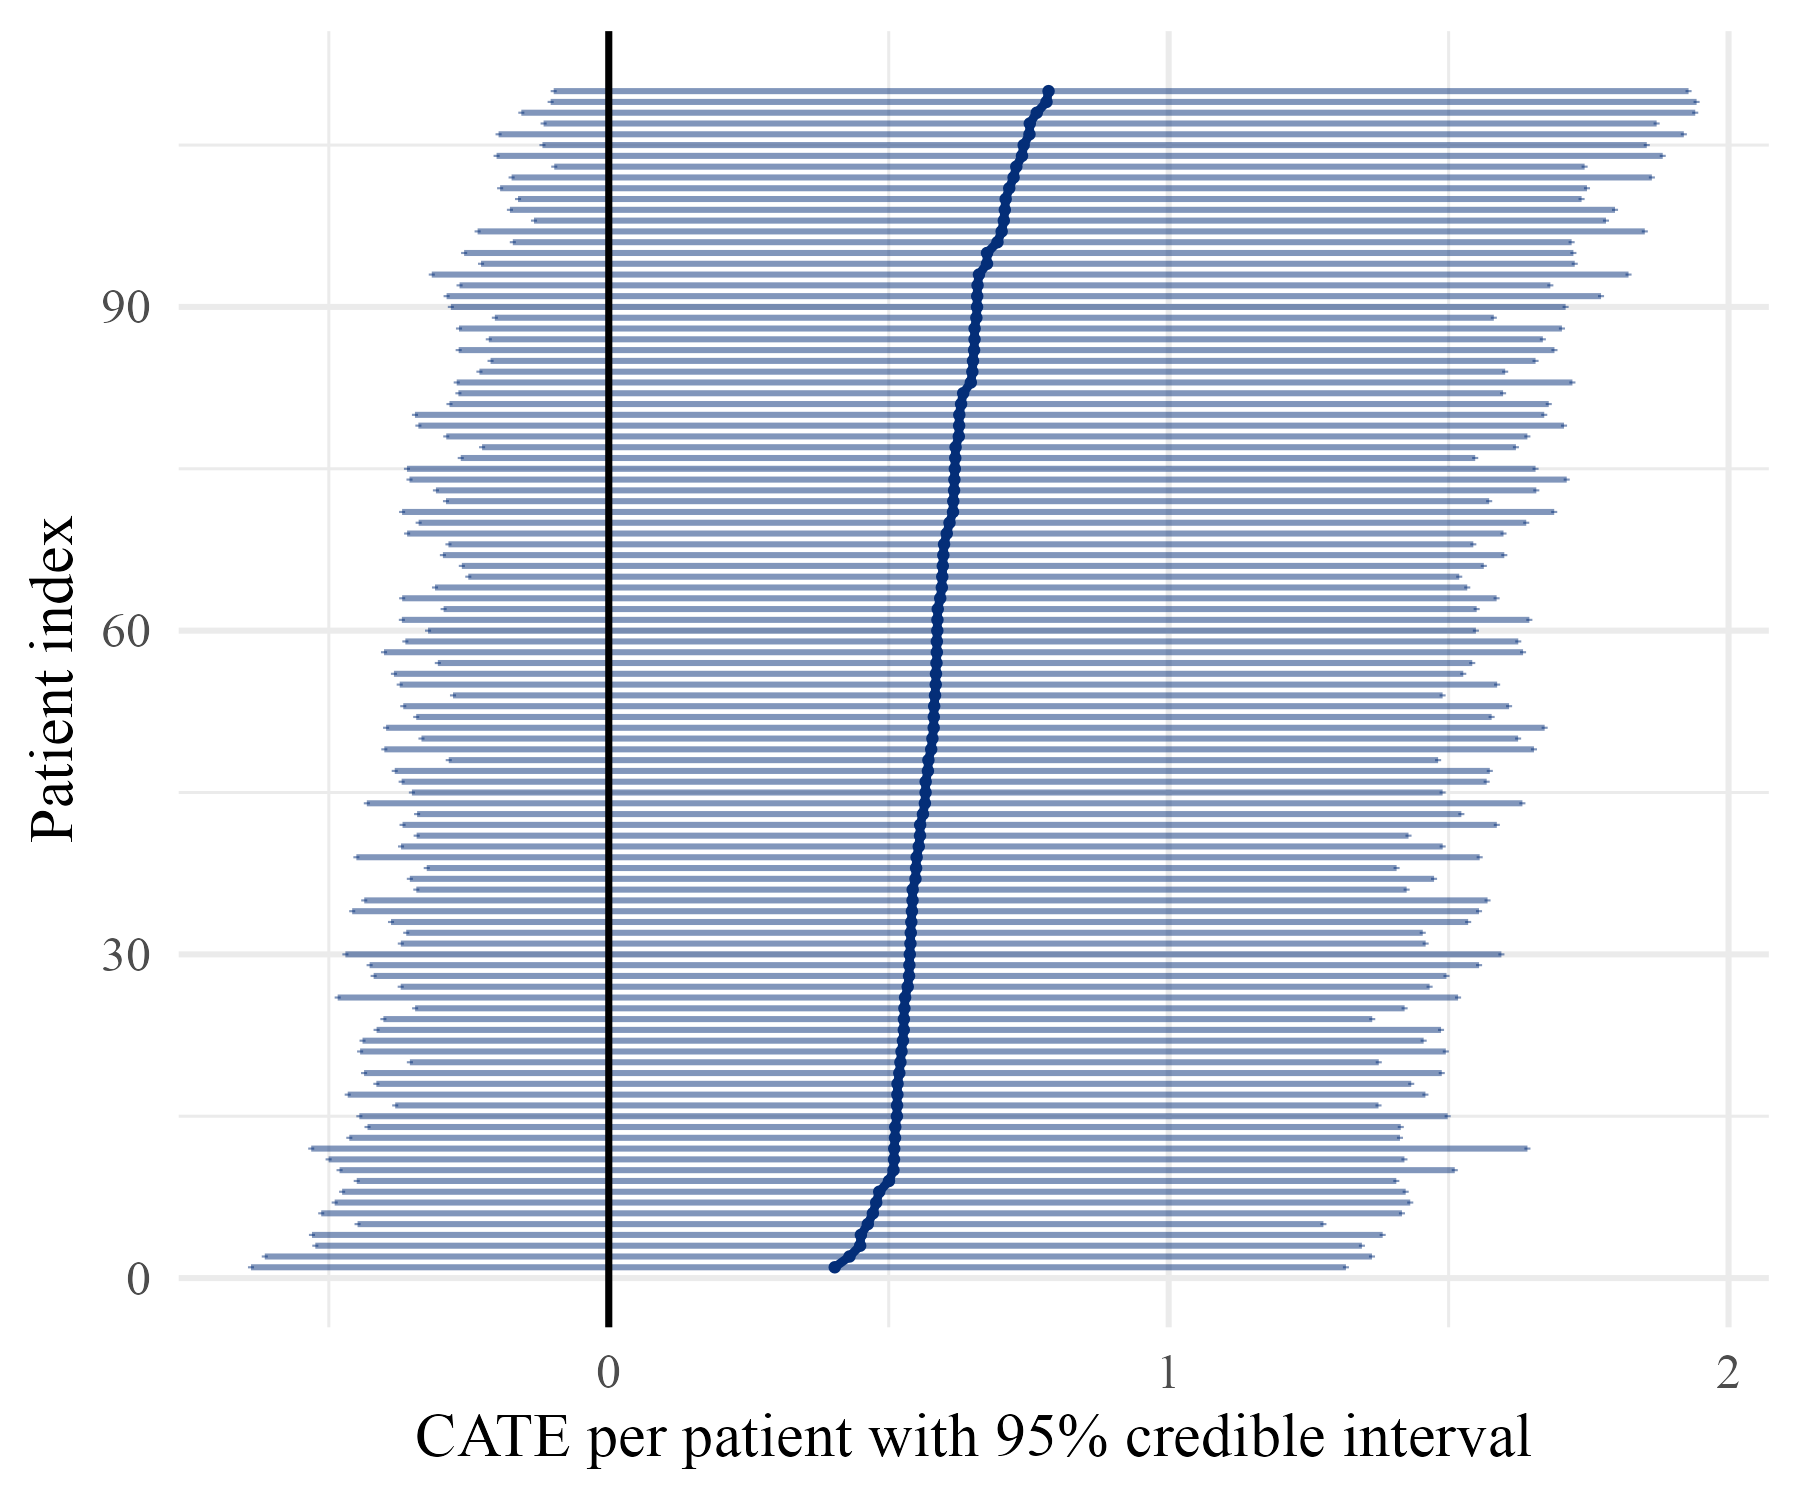
\includegraphics[width=\linewidth]{plot_CATEpatient_Landmark.png}
        \caption{Posterior means and 95\% credible intervals for individual CATEs under adjuvant radiotherapy in patients with PDAC after 6-month landmarking. Patients are sorted by estimated CATE.}
        \label{fig:cate_plot_Landmark}
    \end{minipage}
\end{figure}

